\section{Climate model simulations}
\label{climate}

Daily observations over ten 10-year periods.

Based on the anomalies (DLM).

1990--1999 california winter precipitation, both likelihoods, all three climate model sources, a few thresholds (five?, 0.90 0.92, 0.94, 0.96, 0.98) -> six*five runs

Show mean extremal index

\begin{figure}
\begin{center}
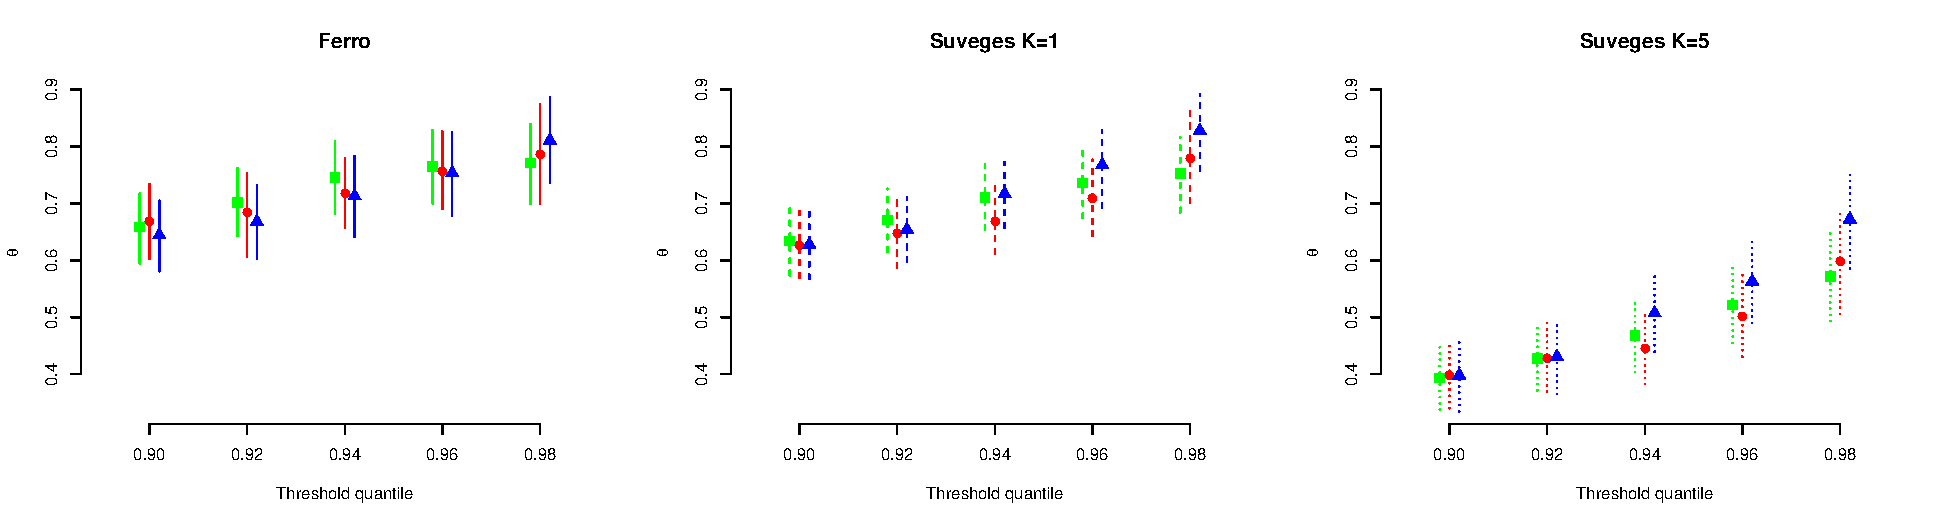
\includegraphics[scale=0.46]{figs/winter_like.pdf}
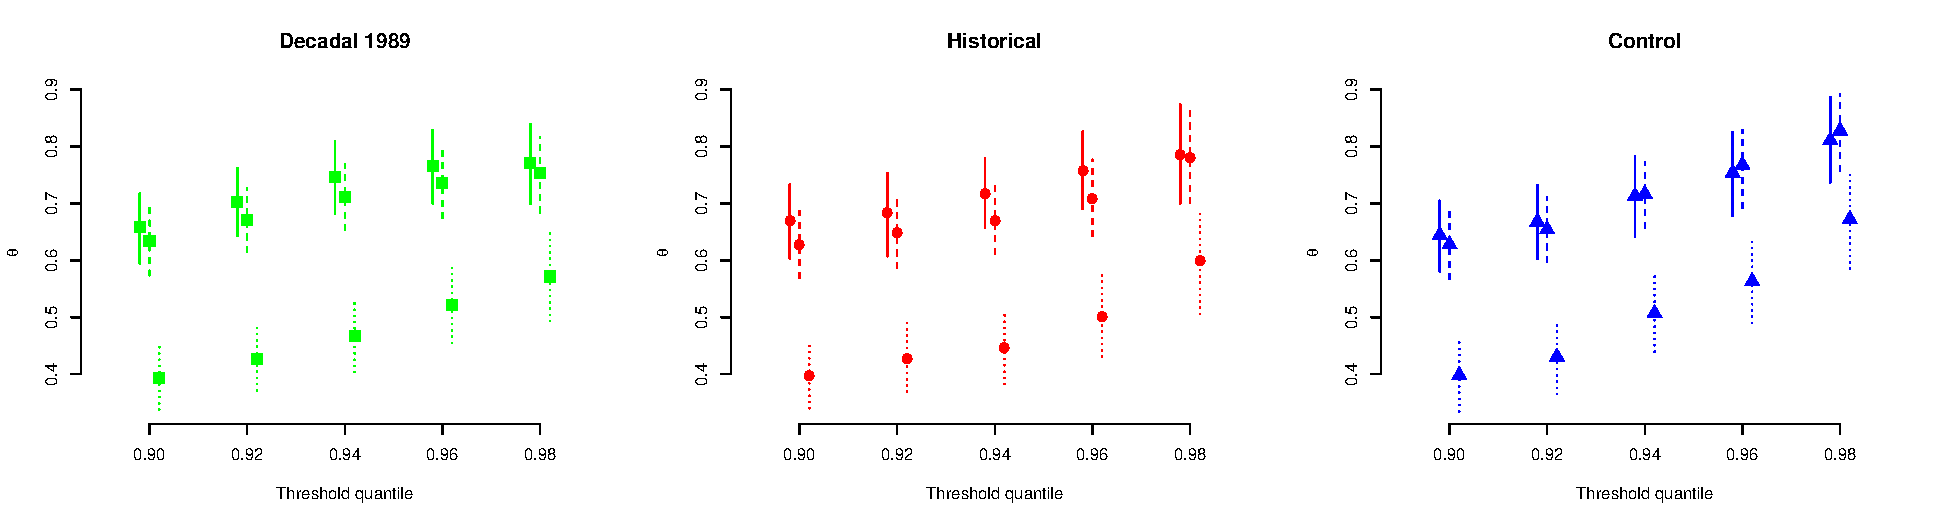
\includegraphics[scale=0.46]{figs/winter_source.pdf}
\end{center}
\caption{Both rows show the same information, but are arranged differently. The top row compares the extremal indexes of the climate models for a given likelihood. The bottom row compares the two likelihoods for each climate model. Solid lines (-----) denote model (\ref{ferro}), dashed lines (- - -) denote model (\ref{suveges}). Squares (\symsquare) mark decadal runs, dots (\symcircle) mark historical runs, and triangles (\symtriangle) are control runs. The points are the posterior means and the lines are 95\% h.p.d. intervals. The domain is California winter precipitation from 1990--1999.}
\label{figwinter}
\end{figure}

\begin{figure}
\begin{center}
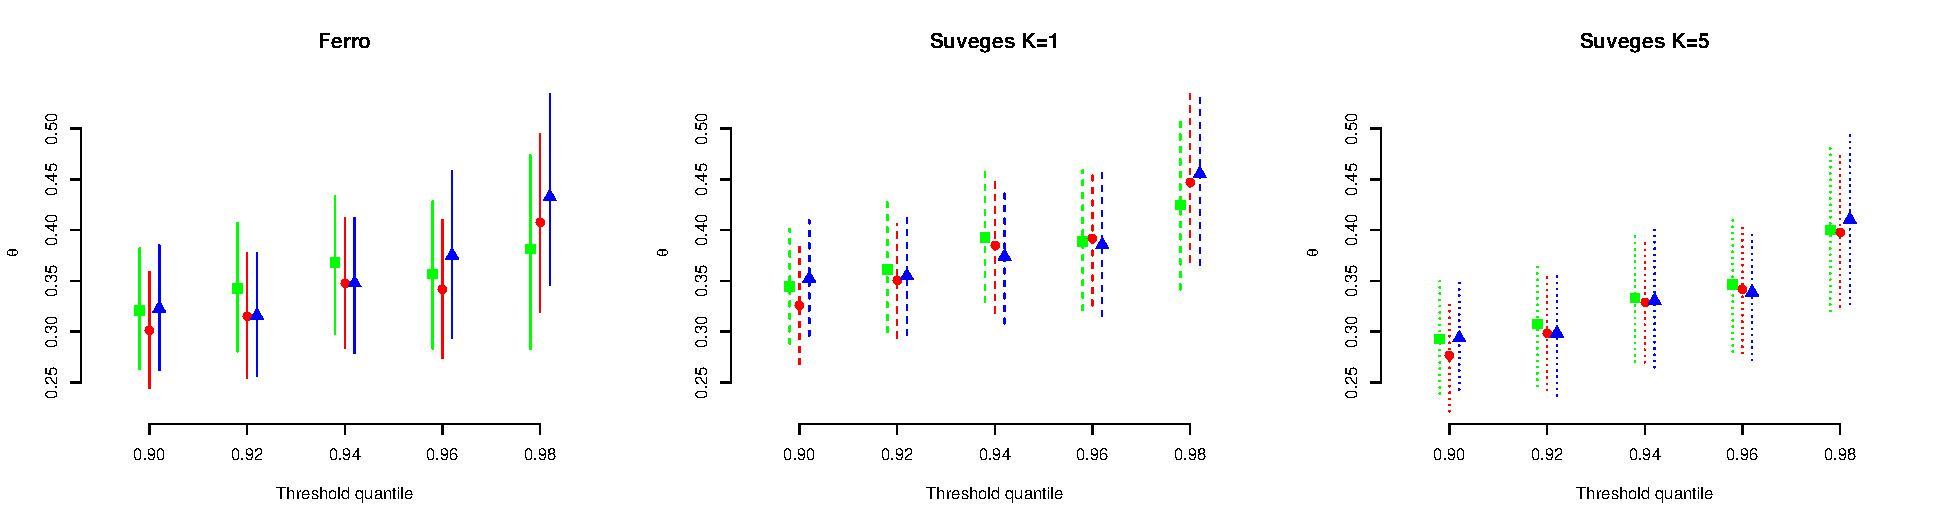
\includegraphics[scale=0.46]{figs/summer_like.pdf}
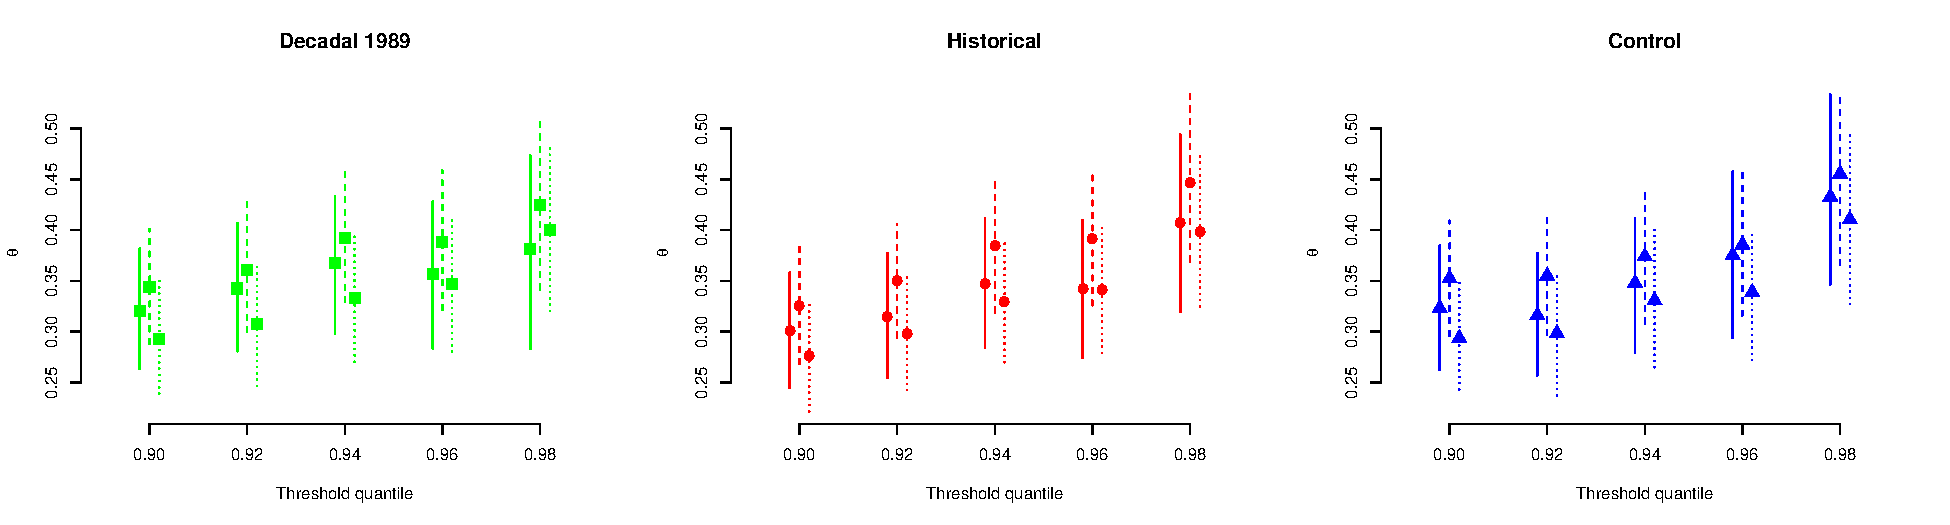
\includegraphics[scale=0.46]{figs/summer_source.pdf}
\end{center}
\caption{Same as in Figure \ref{figwinter}, but the hierarchical model is applied to summer maximum temperature.}
\label{figsummer}
\end{figure}
